\documentclass[journal]{IEEEtran}
\usepackage[a5paper, margin=10mm, onecolumn]{geometry}
\usepackage{amsmath,amssymb}
\usepackage{graphicx}
\usepackage{hyperref}
\usepackage{enumitem}
\begin{document}
	
	\title{10.4.ex17}
	\author{EE24BTECH11022 - ESHAN SHARMA}
	\maketitle
	
	\textbf{Question:}
	A pole has to be erected at a point on the boundary of a circular park of diameter 13 metres in such a way that the difference of its distances from two diametrically opposite fixed gates A and B on the boundary is 7 metres. Is it possible to do so? If yes, at what distances from the two gates should the pole be erected?\\
	
	\textbf{Solution:}
	
	Let the distance of the pole from gate B be \(x\) metres. Then the distance from gate A will be \((x+7)\) metres.
	
	From the Pythagoras theorem, since \(\triangle APB\) is a right triangle:
	\begin{align}
		AB^2 = AP^2 + BP^2
	\end{align}
	Given \(AB = 13\) metres, substituting values:
	\begin{align}
		13^2 &= (x+7)^2 + x^2 \\
		169 &= x^2 + 14x + 49 + x^2 \\
		2x^2 + 14x - 120 &= 0
	\end{align}
	Simplify the equation:
	\begin{align}
		x^2 + 7x - 60 &= 0
	\end{align}
	
	\textbf{Theoretical Solution:}
	Using the quadratic formula \(x = \frac{-b \pm \sqrt{b^2 - 4ac}}{2a}\), where \(a = 1, b = 7, c = -60\):
	\begin{align}
		x &= \frac{-7 \pm \sqrt{7^2 - 4(1)(-60)}}{2(1)} \\
		x &= \frac{-7 \pm \sqrt{289}}{2} \\
		x &= \frac{-7 \pm 17}{2}
	\end{align}
	Thus, \(x = 5\) or \(x = -12\). Since distance cannot be negative, \(x = 5\).
	The distances are:\
	\(BP = 5\) metres, \(AP = 12\) metres.\\
	
	\textbf{Computational Solution: Newton's Method}
	
	Newton's method formula is:
	\begin{align}
		x_{n+1} = x_n - \frac{f(x_n)}{f'(x_n)}
	\end{align}
	Define \(f(x) = x^2 + 7x - 60\) and \(f'(x) = 2x + 7\). The iterative formula becomes:
	\begin{align}
		x_{n+1} = x_n - \frac{x_n^2 + 7x_n - 60}{2x_n + 7}
	\end{align}
	Starting with an initial guess \(x_0 = 0\):
	\begin{align}
		x_1 &= 5 \quad \text{(converges to 5)}
	\end{align}
	Thus, \(x = 5\) is the root.\\
	
	\begin{figure}[h]
	\centering
	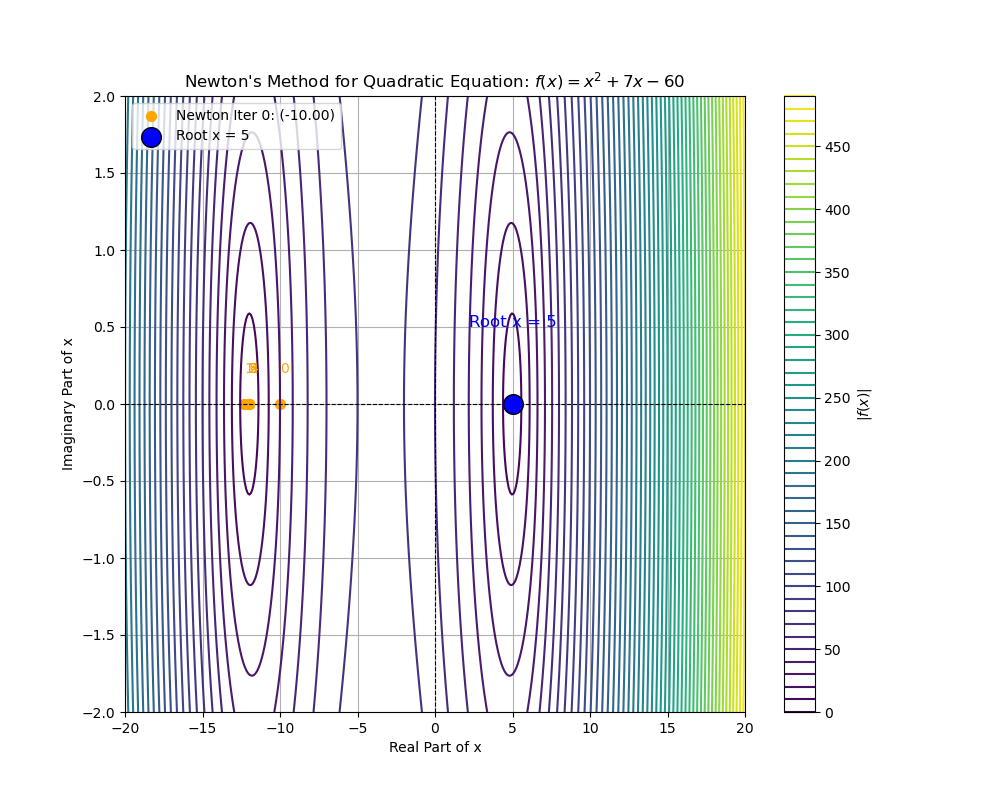
\includegraphics[width=\textwidth]{figs/fig2.png}
	\end{figure}
	
	\textbf{Eigenvalue Solution Using Companion Matrix:}
	
	The quadratic equation \(x^2 + 7x - 60 = 0\) can be solved by finding the eigenvalues of its companion matrix:
	\begin{align}
		A = \begin{bmatrix}
			0 & -60 \\
			1 & -7
		\end{bmatrix}
	\end{align}
	
	\textbf{QR Decomposition Process}\\
	
	\textbf{Step 1: QR Decomposition}\\
	For each iteration, we decompose \( A_k \) into:
	\[
	A_k = Q_k R_k,
	\]
	where:
	\begin{itemize}
		\item \( Q_k \) is an orthogonal matrix, satisfying \( Q_k^\top Q_k = I \),
		\item \( R_k \) is an upper triangular matrix.
	\end{itemize}
	
	\textbf{Step 2: Matrix Updates}\\
	Once the QR decomposition is performed, we update the matrix as:
	\[
	A_{k+1} = R_k Q_k.
	\]
	
	The process is repeated until \( A_k \) converges to an upper triangular matrix \( T \), whose diagonal elements are the eigenvalues of the original matrix.
	
	\textbf{Detailed Steps for QR Decomposition:}\\
	\begin{enumerate}
		\item Start with \( A_0 = A \):
		\[
		A_0 = \begin{bmatrix}
			0 & 60 \\
			1 & -7
		\end{bmatrix}.
		\]
		\item Compute the QR decomposition of \( A_0 \):
		\[
		Q_0 = \begin{bmatrix}
			0 & 1 \\
			1 & 0
		\end{bmatrix}, \quad
		R_0 = \begin{bmatrix}
			1 & -7 \\
			0 & 60
		\end{bmatrix}.
		\]
		\item Update \( A_1 \) as:
		\[
		A_1 = R_0 Q_0 = \begin{bmatrix}
			-7 & 60 \\
			60 & 0
		\end{bmatrix}.
		\]
		\item Repeat the QR decomposition for \( A_1 \):
		\[
		Q_1 = \begin{bmatrix}
			-0.116 & 0.993 \\
			0.993 & 0.116
		\end{bmatrix}, \quad
		R_1 = \begin{bmatrix}
			-60.57 & 6.93 \\
			0 & 60.28
		\end{bmatrix}.
		\]
		\item Update \( A_2 \):
		\[
		A_2 = R_1 Q_1 = \begin{bmatrix}
			-6.93 & 60.28 \\
			60.28 & 0.57
		\end{bmatrix}.
		\]
	\end{enumerate}
	
	\textbf{Final Step: Convergence}\\
	This iterative process is continued until \( A_k \) becomes an upper triangular matrix:
	\[
	T = \begin{bmatrix}
		5 & 0 \\
		0 & -12
	\end{bmatrix}.
	\]
	
	The eigenvalues of \( T \) are \( \lambda_1 = 5 \) and \( \lambda_2 = -12 \), which are the roots of the original quadratic equation.
	
	Thus, the solution is \(x = 5\).\\
	
	\begin{figure}[h]
		\centering
		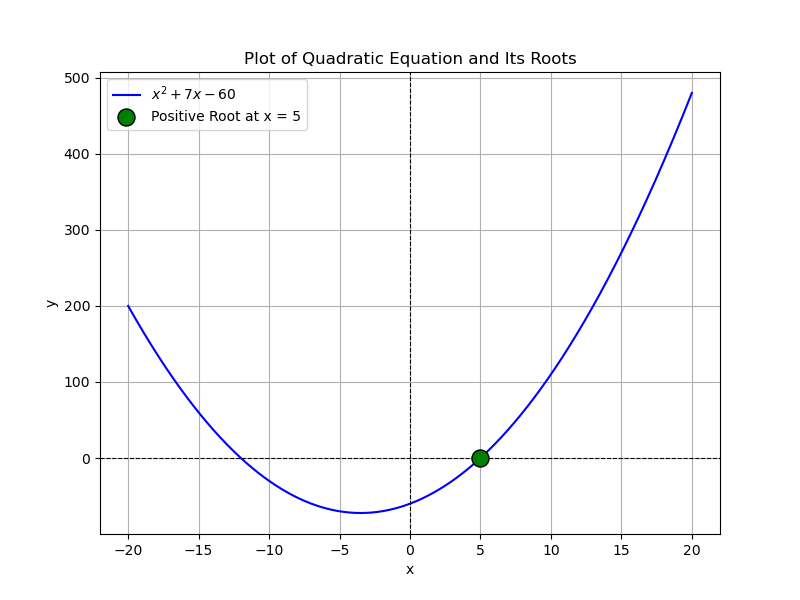
\includegraphics[width=\textwidth]{figs/fig.png}
	\end{figure}
	
	\textbf{Conclusion:}
	The pole can be erected at distances of 5 metres from gate B and 12 metres from gate A.
	
\end{document}
